% Бүлэг 2

\chapter{Ажил горилогчийн ур чадварыг үнэлэх системийн шинжилгээ} % Бүлгийн нэр
\label{Chapter2} % Энэ бүлэг рүү ишлэл хийх бол \ref{Chapter1} командыг ашигла 

\section{Системийн үйл ажиллагааны тухай дэлгэрэнгүй}
\subsection*{User scenario}
\subsection*{Ажил горилогч}
\par{} Системд өөрийн бүртгэлээр нэвтрэн орно. Ажлын байруудын жагсаалтуудыг харах бөгөөд сонирхож буй ажлын байрыг сонгон орж, шалгууруудтай танилцана. Хэрэв тухайн ажлын байрыг сонирхож байвал өөрийн анкетыг явуулж, шалгуурт хэр нийцэж байгааг шалгуулна. Анкетыг үнэлж дууссаны дараа чадвар болгоныг үнэлсэн хариу гарах бөгөөд үүнд шалгуурт таарсан болон тэнцээгүй чадваруудыг яагаад гэдгийг тайлбарлан харуулна. Хэрэв өөрийгөө хангалттай гэж үзвэл ажилд орох хүсэлт буюу анкетийг явуулна. Ур чадвар хангалттай хэмжээнд тэнцсэн гэж ажил олгогч үзсэн тохиолдолд дараагийн шатны даалгаврыг явуулсан үед өгөгдсөн хугацаанд хийж явуулж болно. Мөн хэрэглэгч чат боттой харьцан, өөрийн хүсэмжит цалингийн хэмжээ, байршил зэргээс хамааран өөрт хамгийн тохиромжтой ажлын байрыг олох боломжтой. 
\subsection*{Ажил олгогч (Хүний нөөц)} 
\par{} Системд нэвтрэн орсны дараа ажлын байрны саналыг оруулах бөгөөд үүний дараа шалгуурыг оруулж өгнө. Тухайн ажлын байранд ирсэн хүсэлтүүдийг харж болох ба тэнцсэн хувь болон тухайн ажилтны үнэ цэн дээр тулгуурлан шүүнэ. Амжилттай шалгууруудыг давсан хүмүүст шаардлагатай гэж үзвэл дараагийн шатны даалгаврыг илгээх ба даалгаврыг хиймэл оюунаар эсвэл хүний нөөц өөрсдөө үүсгэх, мөн шаардлагатай тохиолдолд засах боломжтой. Ажил горилогчдын гүйцэтгэж илгээсэн даалгаврыг харах боломжтой байна. Хэрэв аль нэг ажил горилогчийг сонирхож байвал дараагийн уулзалтад цаг товлоно. 
\subsection*{AI} 
\par{}Ажил горилогчийн CV-г тухайн ажлын байрны шаардлагатай харьцуулж, нийцлийг тодорхойлно. Үүний тулд Anthropic Claude API (LLM)-г ашиглан CV-ийн текстийг задлаж, тохирсон болон дутуу ур чадваруудыг тайлбарлах (explainable) үнэлгээ гаргана. Чатботод RAG (Retrieval-Augmented Generation) аргачлалыг хэрэгжүүлсэн бөгөөд өгөгдлийн сангаас идэвхтэй ажлын байрны мэдээллийг олж авч, Claude API-д контекст болгон дамжуулж хариулт үүсгэнэ. Мөн ажил олгогчийн хүсэлтээр ажлын байрны шаардлагад тулгуурлан AI-аар даалгавар автоматаар үүсгэх үйлчилгээ хэрэгжинэ.

\section{Системийг ашиглах хэрэглэгчид}
\begin{enumerate}
    \item  Ажил горилогч
    \item  Ажил олгогч буюу байгууллагын хүний нөөц
\end{enumerate}
\section{Функциональ шаардлага}
\subsection*{Ажил олгогчийн функциональ шаардлага}
\begin{enumerate}
\item Системд нэвтрэх
\item Ажлын байрны зар шинээр үүсгэх, засах, устгах
\item Ажлын зар бүрт шаардлага (ур чадвар, туршлага, цалин, байршил) тодорхойлох
\item Ажлын байрны жагсаалтыг харах, удирдах
\item Ирсэн анкетуудыг харах
\item Анкет бүрийн AI үнэлгээ болон тохирох хувийг харах
\item Ажил горилогчдыг шүүх, эрэмбэлэх
\item AI ашиглан даалгавар үүсгэх
\item Даалгавар үүсгэх, засах, илгээх
\item Илгээсэн даалгаврын гүйцэтгэлийг харах
\item Даалгаврын гүйцэтгэлд үндэслэн үнэлгээ өгөх
\item Ярилцлагын цаг товлох
\end{enumerate}

\subsection*{Ажил горилогчийн функциональ шаардлага}
\begin{enumerate}
\item Системд нэвтрэх
\item Хувийн мэдээлэл засах
\item Ажлын байр хайх
\item Ажлын байрны дэлгэрэнгүй мэдээлэл харах
\item Ажлын байранд анкет илгээх
\item Анкетын AI үнэлгээ болон чадварын дүнг харах
\item Дутуу чадварууд болон сайжруулах зөвлөмж харах
\item Даалгавар хүлээн авах
\item Даалгавар гүйцэтгэж илгээх
\item Илгээсэн даалгаврын төлөв харах
\item Чатботтой харилцах (ажлын санал авах)
\item Өөрт тохирсон ажлын санал (recommendation) авах
\end{enumerate}
\subsection*{Системийн функциональ шаардлага}
\begin{enumerate}
\item Хэрэглэгчийн эрх (authorization) удирдах
\item CV/анкетаас мэдээллийг задалж авах
\item Ажлын шаардлагыг илгээсэн анкеттай тааруулж, оноог тооцоолох
\item Чадвар тус бүр дээр үнэлгээ гаргаж, шалтгааныг тайлбарлах
\item Тохирох ажлын байрыг санал болгох
\item Даалгаврын чанарыг шалгах
\item Notification system (даалгавар, ярилцлага)
\item File upload (CV, даалгавар) хадгалах
\end{enumerate}
\section{Функциональ бус шаардлага} %TODO

\begin{itemize}
    \item Энгийн хуудас (нэвтрэх, ажлын зарын жагсаалт) 2 секундын дотор ачаалагдах.
    \item Анкетын AI үнэлгээ (Claude API дуудлага)-ний хариу 5--15 секундын дотор гарж ирэх.
    \item Чатботын RAG хариулт 3--5 секундын дотор гарах.
    \item Өгөгдлийн сангийн нэг үйлдлийн дундаж хариу 200мс-ээс хэтрэхгүй байх.
    \item Систем зэрэг 200 идэвхтэй хэрэглэгчийг дэмжих чадвартай байх.
    \item AI үйлчилгээний дуудлагыг дараалалд (queue) оруулж, ачаалал ихсэх үед тогтвортой ажиллах.
    \item Хэрэглэгчийн нууц үгийг bcrypt алгоритмаар хэшлэн хадгалах.
    \item Системд нэвтрэхэд JWT (JSON Web Token) ашиглан session удирдах.
    \item Үүрэгт суурилсан эрхийн хяналт тавих.
    \item Бүх API дуудлага HTTPS дамжуулалттай байх.
    \item SQL injection, XSS, CSRF халдлагаас хамгаалах.
    \item Системийн бэлэн байдал (uptime) сард 97\% буюу түүнээс дээш байх.
    \item Claude API саатах эсвэл алдаа гаргах тохиолдолд хэрэглэгчид ойлгомжтой алдааны мэдээлэл харуулж, дараа дахин оролдох боломж олгох.
    \item Өгөгдлийн сангийн нөөцлөлтийг 7 хоногт нэг удаа автоматаар хийх.
    \item Интерфэйс монгол хэл дээр, ойлгомжтой цэстэй байх.
    \item AI үнэлгээний үр дүнг тоон оноо болон тайлбартайгаар (explainable) харуулах.
\end{itemize}
\section{Юзкейс диаграмм}
\paragraph{} Зураг \ref{fig:usecase} -д дүрслэгдсэн уг юзкейс диаграмм нь зочин, ажил олгогч болон горилогч гэсэн тоглогчид болон тэдгээрийн ашиглаж болон нийт 12 юзкейсыг агуулсан.
\subsection* {\textbf{Actors:}}
    \begin{itemize}
        \item Ажил олгогч
        \item Ажил горилогч
        \item Зочин
    \end{itemize} 
\subsection*{ \textbf{Use cases:}}
    \par{} \textbf{Зочин}
        \begin{itemize}
        \item Ажил горилогчоор бүртгүүлэх
        \item Ажил олгогчоор бүртгүүлэх
    \end{itemize}
    \par{} \textbf{Ажил горилогч}
    \begin{itemize}
        \item Ажлын зар харах
        \item Анкет илгээх % <<include>> AI үнэлгээ харах
        \item AI үнэлгээ харах 
        \item Даалгавар гүйцэтгэх
        \item Чатботтой харилцах
    \end{itemize}

    \par{} \textbf{Ажил олгогч}
    \begin{itemize}
        \item Ажлын байрны зар удирдах
        \item Ирсэн анкетуудыг харах
        \item Уулзалт товлох
        \item Даалгаврыг удирдах
        \item Даалгаврын гүйцэтгэлийг харах, үнэлэх
    \end{itemize}
\begin{figure}[H]
    \centering
    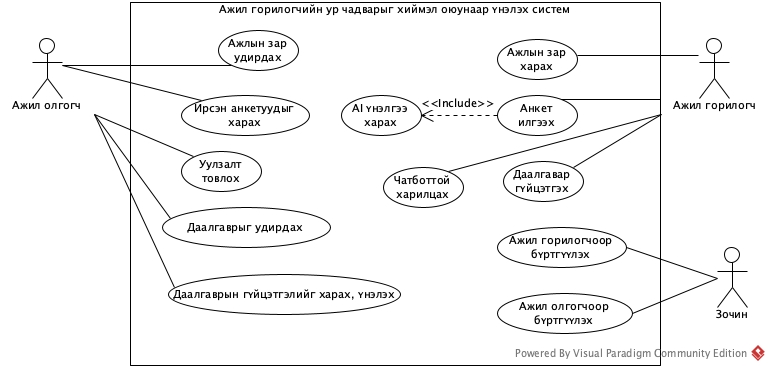
\includegraphics[scale=0.55]{Figures/chapter2/Use Case Diagram1.jpg}
    \caption{Юзкейс диаграмм}
    \label{fig:usecase}
\end{figure}
\section{Юзкейсийн тодорхойлолт}
\begin{longtable}{|r|p{11.5cm}|}
    \caption{Ажил горилогчоор бүртгүүлэх юзкейсийн тодорхойлолт}
    \label{table:usecase1}\\ \hline
    {Юзкейс:} & {Ажил горилогчоор бүртгүүлэх}\\ \hline
    {ID:} & {1}\\ \hline
    {Үүсгэсэн:} & {Ц. Анужин}\\ \hline
    {Үүсгэсэн огноо:} & {2025-03-21}\\ \hline
    {Үндсэн тоглогч:} & {Зочин}\\ \hline
    {Нэмэлт тоглогч:} & {Байхгүй}\\ \hline
    {Товч тайлбар:} & {Зочин системд ажил горилогчоор бүртгүүлнэ.}\\ \hline
    {Өмнөх нөхцөл:} & {Байхгүй}\\ \hline
    {Үндсэн урсгал:} & {\begin{enumerate}[nosep]
        \item Зочин ажил горилогчоор бүртгүүлэх үйлдлийг сонгоно.
        \item Бүртгэлийн мэдээллээ оруулна.
        \item Систем мэдээллийг шалгаж бүртгэл үүсгэнэ.
    \end{enumerate}}\\ \hline
    {Дараах нөхцөл:} & {\begin{enumerate}[nosep]
        \item Зочин системд ажил горилогчоор бүртгэгдсэн байна.
    \end{enumerate}}\\ \hline
    {Альтернатив урсгал:} & {Байхгүй}\\ \hline
\end{longtable}

\begin{longtable}{|r|p{11.5cm}|}
    \caption{Ажил олгогчоор бүртгүүлэх юзкейсийн тодорхойлолт}
    \label{table:usecase2}\\ \hline
    {Юзкейс:} & {Ажил олгогчоор бүртгүүлэх}\\ \hline
    {ID:} & {2}\\ \hline
    {Үүсгэсэн:} & {Ц. Анужин}\\ \hline
    {Үүсгэсэн огноо:} & {2025-03-21}\\ \hline
    {Үндсэн тоглогч:} & {Зочин}\\ \hline
    {Нэмэлт тоглогч:} & {Байхгүй}\\ \hline
    {Товч тайлбар:} & {Зочин системд ажил олгогчоор бүртгүүлнэ.}\\ \hline
    {Өмнөх нөхцөл:} & {Байхгүй}\\ \hline
    {Үндсэн урсгал:} & {\begin{enumerate}[nosep]
        \item Зочин ажил олгогчоор бүртгүүлэх үйлдлийг сонгоно.
        \item Байгууллага болон бүртгэлийн мэдээллээ оруулна.
        \item Систем мэдээллийг шалгаж ажил олгогчийн бүртгэл үүсгэнэ.
    \end{enumerate}}\\ \hline
    {Дараах нөхцөл:} & {\begin{enumerate}[nosep]
        \item Зочин системд ажил олгогчоор бүртгэгдсэн байна.
    \end{enumerate}}\\ \hline
    {Альтернатив урсгал:} & {Байхгүй}\\ \hline
\end{longtable}

\begin{longtable}{|r|p{11.5cm}|}
    \caption{Ажлын зар харах юзкейсийн тодорхойлолт}
    \label{table:usecase3}\\ \hline
    {Юзкейс:} & {Ажлын зар харах}\\ \hline
    {ID:} & {3}\\ \hline
    {Үүсгэсэн:} & {Ц. Анужин}\\ \hline
    {Үүсгэсэн огноо:} & {2025-03-21}\\ \hline
    {Үндсэн тоглогч:} & {Ажил горилогч}\\ \hline
    {Нэмэлт тоглогч:} & {Байхгүй}\\ \hline
    {Товч тайлбар:} & {Ажил горилогч нийтлэгдсэн ажлын байруудын жагсаалтыг харж, шүүлт ашиглан хайлт хийнэ.}\\ \hline
    {Өмнөх нөхцөл:} & {\begin{enumerate}[nosep]
        \item Ажил горилогч системд нэвтэрсэн байна.
        \item Системд нийтлэгдсэн ажлын зар байна.
    \end{enumerate}}\\ \hline
    {Үндсэн урсгал:} & {\begin{enumerate}[nosep]
        \item Ажил горилогч ажлын зарын жагсаалтын хуудас руу орно.
        \item Систем нийтлэгдсэн ажлын заруудыг харуулна.
        \item Ажил горилогч байршил, цалин, чиглэлээр шүүлт хийнэ.
        \item Систем шүүлтэд тохирсон заруудыг харуулна.
        \item Ажил горилогч сонирхсон зараа дарж дэлгэрэнгүй мэдээллийг харна.
    \end{enumerate}}\\ \hline
    {Дараах нөхцөл:} & {\begin{enumerate}[nosep]
        \item Ажил горилогч ажлын байрны дэлгэрэнгүй мэдээллийг харсан байна.
    \end{enumerate}}\\ \hline
    {Альтернатив урсгал:} & {Байхгүй}\\ \hline
\end{longtable}

\begin{longtable}{|r|p{11.5cm}|}
    \caption{Анкет илгээх юзкейсийн тодорхойлолт}
    \label{table:usecase4}\\ \hline
    {Юзкейс:} & {Анкет илгээх}\\ \hline
    {ID:} & {4}\\ \hline
    {Үүсгэсэн:} & {Ц. Анужин}\\ \hline
    {Үүсгэсэн огноо:} & {2025-03-21}\\ \hline
    {Үндсэн тоглогч:} & {Ажил горилогч}\\ \hline
    {Нэмэлт тоглогч:} & {Байхгүй}\\ \hline
    {Товч тайлбар:} & {Ажил горилогч сонгосон ажлын байранд CV/анкетаа илгээх бөгөөд систем автоматаар AI үнэлгээг дуусгана. \textit{(<<include>> AI үнэлгээ харах)}}\\ \hline
    {Өмнөх нөхцөл:} & {\begin{enumerate}[nosep]
        \item Ажил горилогч системд нэвтэрсэн байна.
        \item Ажил горилогч ажлын байрны дэлгэрэнгүй хуудсыг нээсэн байна.
    \end{enumerate}}\\ \hline
    {Үндсэн урсгал:} & {\begin{enumerate}[nosep]
        \item Ажил горилогч "Анкет илгээх" товчийг дарна.
        \item Систем CV файл хуулах форм харуулна.
        \item Ажил горилогч CV файлаа сонгоно.
        \item "Илгээх" товчийг дарна.
        \item Систем файлыг хадгалж AI-д дамжуулна.
        \item include (AI үнэлгээ харах)
    \end{enumerate}}\\ \hline
    {Дараах нөхцөл:} & {\begin{enumerate}[nosep]
        \item Анкет системд хадгалагдсан байна.
        \item AI үнэлгээ автоматаар үүссэн байна.
    \end{enumerate}}\\ \hline
    {Альтернатив урсгал:} & {Байхгүй}\\ \hline
\end{longtable}

\begin{longtable}{|r|p{11.5cm}|}
    \caption{AI үнэлгээ харах юзкейсийн тодорхойлолт}
    \label{table:usecase5}\\ \hline
    {Юзкейс:} & {AI үнэлгээ харах}\\ \hline
    {ID:} & {5}\\ \hline
    {Үүсгэсэн:} & {Ц. Анужин}\\ \hline
    {Үүсгэсэн огноо:} & {2025-03-21}\\ \hline
    {Үндсэн тоглогч:} & {Ажил горилогч}\\ \hline
    {Нэмэлт тоглогч:} & {Байхгүй}\\ \hline
    {Товч тайлбар:} & {Ажил горилогч анкет илгээсний дараа AI үнэлгээ болон чадварын дүнг тооцоолон гаргаж, сайжруулах зөвлөмжийг харуулна.}\\ \hline
    {Өмнөх нөхцөл:} & {\begin{enumerate}[nosep]
        \item Анкетын мэдээллийг хүлээж авсан байна.
    \end{enumerate}}\\ \hline
    {Үндсэн урсгал:} & {\begin{enumerate}[nosep]
        \item Систем анкетын мэдээлэл болон ажлын байрны мэдээллийг харьцуулан, дүн шинжилгээ хийж, үнэлгээг гаргана.
        \item Систем ажил горилогчид AI үнэлгээний дүнг харуулна.
        \item Ажил горилогч тэнцсэн болон тэнцээгүй чадваруудын тайлбарыг харна.
        \item Ажил горилогч дутуу чадваруудыг сайжруулах зөвлөмжийг харна.
    \end{enumerate}}\\ \hline
    {Дараах нөхцөл:} & {\begin{enumerate}[nosep]
        \item AI үнэлгээ амжилттай хийгдсэн байна.
        \item Ажил горилогч өөрийн анкетын үнэлгээтэй танилцсан байна.
    \end{enumerate}}\\ \hline
    {Альтернатив урсгал:} & {Байхгүй}\\ \hline
\end{longtable}

\begin{longtable}{|r|p{11.5cm}|}
    \caption{Даалгавар гүйцэтгэх юзкейсийн тодорхойлолт}
    \label{table:usecase6}\\ \hline
    {Юзкейс:} & {Даалгавар гүйцэтгэх}\\ \hline
    {ID:} & {6}\\ \hline
    {Үүсгэсэн:} & {Ц. Анужин}\\ \hline
    {Үүсгэсэн огноо:} & {2025-03-21}\\ \hline
    {Үндсэн тоглогч:} & {Ажил горилогч}\\ \hline
    {Нэмэлт тоглогч:} & {Байхгүй}\\ \hline
    {Товч тайлбар:} & {Ажил горилогч ажил олгогчоос хүлээн авсан даалгаврыг гүйцэтгэж системд буцааж илгээнэ.}\\ \hline
    {Өмнөх нөхцөл:} & {\begin{enumerate}[nosep]
        \item Ажил горилогч системд нэвтэрсэн байна.
        \item Ажил олгогч даалгаврыг илгээсэн байна.
        \item Даалгаврын хугацаа дуусаагүй байна.
    \end{enumerate}}\\ \hline
    {Үндсэн урсгал:} & {\begin{enumerate}[nosep]
        \item Ажил горилогч мэдэгдлийг хүлээн авч даалгаврын хуудас руу орно.
        \item Систем даалгаврын дэлгэрэнгүй мэдээлэл болон хугацааг харуулна.
        \item Ажил горилогч даалгаврыг уншиж гүйцэтгэнэ.
        \item Гүйцэтгэлийн файл эсвэл хариултыг системд хуулна.
        \item "Илгээх" товчийг дарна.
        \item Даалгаврын төлөв "Илгээгдсэн" болж өөрчлөгдөнө.
    \end{enumerate}}\\ \hline
    {Дараах нөхцөл:} & {\begin{enumerate}[nosep]
        \item Даалгаврын гүйцэтгэл системд хадгалагдсан байна.
        \item Ажил олгогч гүйцэтгэлийг харах боломжтой болсон байна.
    \end{enumerate}}\\ \hline
    {Альтернатив урсгал:} & {}\\ \hline
\end{longtable}

\begin{longtable}{|r|p{11.5cm}|}
    \caption{Чатботтой харилцах юзкейсийн тодорхойлолт}
    \label{table:usecase7}\\ \hline
    {Юзкейс:} & {Чатботтой харилцах}\\ \hline
    {ID:} & {7}\\ \hline
    {Үүсгэсэн:} & {Ц. Анужин}\\ \hline
    {Үүсгэсэн огноо:} & {2025-03-21}\\ \hline
    {Үндсэн тоглогч:} & {Ажил горилогч}\\ \hline
    {Нэмэлт тоглогч:} & {Байхгүй}\\ \hline
    {Товч тайлбар:} & {Ажил горилогч AI чатботтой харьцан өөрт тохирсон ажлын байрны саналыг авна.}\\ \hline
    {Өмнөх нөхцөл:} & {\begin{enumerate}[nosep]
        \item Ажил горилогч системд нэвтэрсэн байна.
    \end{enumerate}}\\ \hline
    {Үндсэн урсгал:} & {\begin{enumerate}[nosep]
        \item Ажил горилогч чатботын хуудас руу орно.
        \item Ажил горилогч өөрийн хүссэн цалин, байршил, чиглэлийн талаар мэдээлэл оруулна.
        \item AI хэрэглэгчийн хүсэлтийг боловсруулна.
        \item Систем тохирох ажлын байруудыг санал болгоно.
        \item Ажил горилогч санал болгосон ажлын байруудтай танилцана.
        \item Ажил горилогч нэмэлт асуулт тавих эсвэл харилцааг үргэлжлүүлж болно.
    \end{enumerate}}\\ \hline
    {Дараах нөхцөл:} & {\begin{enumerate}[nosep]
        \item Ажил горилогч өөрт тохирсон ажлын байрны мэдээллийг авсан байна.
    \end{enumerate}}\\ \hline
    {Альтернатив урсгал:} & {Байхгүй}\\ \hline
\end{longtable}

\begin{longtable}{|r|p{11.5cm}|}
    \caption{Ажлын байрны зар удирдах юзкейсийн тодорхойлолт}
    \label{table:usecase8}\\ \hline
    {Юзкейс:} & {Ажлын байрны зар удирдах}\\ \hline
    {ID:} & {8}\\ \hline
    {Үүсгэсэн:} & {Ц. Анужин}\\ \hline
    {Үүсгэсэн огноо:} & {2025-03-21}\\ \hline
    {Үндсэн тоглогч:} & {Ажил олгогч}\\ \hline
    {Нэмэлт тоглогч:} & {Байхгүй}\\ \hline
    {Товч тайлбар:} & {Ажил олгогч ажлын байрны зарыг шинээр үүсгэх, засах, устгах үйлдлүүдийг гүйцэтгэнэ.}\\ \hline
    {Өмнөх нөхцөл:} & {\begin{enumerate}[nosep]
        \item Ажил олгогч системд нэвтэрсэн байна.
    \end{enumerate}}\\ \hline
    {Үндсэн урсгал:} & {\begin{enumerate}[nosep]
        \item Ажил олгогч ажлын зарын удирдлагын хуудас руу орно.
        \item \textbf{if} Шинэ зар үүсгэх бол
            \begin{enumerate}[nosep,label*=\arabic*.]
                \item "Шинэ зар үүсгэх" товчийг дарна.
                \item Ажлын байрны нэр, шаардлага, цалин, байршлыг оруулна.
                \item "Хадгалах" товчийг дарна.
                \item Зар нийтлэгдэнэ.
            \end{enumerate}
        \item \textbf{if} Зар засах бол
            \begin{enumerate}[nosep,label*=\arabic*.]
                \item Засах зарыг сонгоод "Засах" товчийг дарна.
                \item Мэдээллийг өөрчилж "Хадгалах" товчийг дарна.
            \end{enumerate}
        \item \textbf{if} Зар устгах бол
            \begin{enumerate}[nosep,label*=\arabic*.]
                \item Устгах зарыг сонгоод "Устгах" товчийг дарна.
                \item Систем баталгаажуулах цонх харуулна.
                \item Ажил олгогч баталгаажуулна.
                \item Зар устгагдана.
            \end{enumerate}
    \end{enumerate}}\\ \hline
    {Дараах нөхцөл:} & {\begin{enumerate}[nosep]
        \item Ажлын зарт хийсэн өөрчлөлт системд хадгалагдсан байна.
    \end{enumerate}}\\ \hline
    {Альтернатив урсгал:} & {Байхгүй}\\ \hline
\end{longtable}

\begin{longtable}{|r|p{11.5cm}|}
    \caption{Ирсэн анкетуудыг харах юзкейсийн тодорхойлолт}
    \label{table:usecase9}\\ \hline
    {Юзкейс:} & {Ирсэн анкетуудыг харах}\\ \hline
    {ID:} & {9}\\ \hline
    {Үүсгэсэн:} & {Ц. Анужин}\\ \hline
    {Үүсгэсэн огноо:} & {2025-03-21}\\ \hline
    {Үндсэн тоглогч:} & {Ажил олгогч}\\ \hline
    {Нэмэлт тоглогч:} & {Байхгүй}\\ \hline
    {Товч тайлбар:} & {Ажил олгогч тухайн ажлын байранд ирсэн анкетуудыг AI үнэлгээний дүнтэй хамт харж шүүнэ.}\\ \hline
    {Өмнөх нөхцөл:} & {\begin{enumerate}[nosep]
        \item Ажил олгогч системд нэвтэрсэн байна.
        \item Тухайн ажлын байранд анкет ирсэн байна.
    \end{enumerate}}\\ \hline
    {Үндсэн урсгал:} & {\begin{enumerate}[nosep]
        \item Ажил олгогч ажлын зарыг сонгоно.
        \item Систем ирсэн анкетуудын жагсаалтыг тохирох хувиар эрэмбэлж харуулна.
        \item Ажил олгогч анкет бүрийн дэлгэрэнгүй үнэлгээг харна.
        \item Ажил олгогч шаардлагатай бол нэмэлт шүүлт хийнэ.
    \end{enumerate}}\\ \hline
    {Дараах нөхцөл:} & {\begin{enumerate}[nosep]
        \item Ажил олгогч анкетуудтай танилцаж дараагийн шатны шийдвэр гаргахад бэлэн байна.
    \end{enumerate}}\\ \hline
    {Альтернатив урсгал:} & {Байхгүй}\\ \hline
\end{longtable}

\begin{longtable}{|r|p{11.5cm}|}
    \caption{Уулзалт товлох юзкейсийн тодорхойлолт}
    \label{table:usecase10}\\ \hline
    {Юзкейс:} & {Уулзалт товлох}\\ \hline
    {ID:} & {10}\\ \hline
    {Үүсгэсэн:} & {Ц. Анужин}\\ \hline
    {Үүсгэсэн огноо:} & {2025-03-21}\\ \hline
    {Үндсэн тоглогч:} & {Ажил олгогч}\\ \hline
    {Нэмэлт тоглогч:} & {Ажил горилогч}\\ \hline
    {Товч тайлбар:} & {Ажил олгогч сонирхсон ажил горилогчтойгоо ярилцлагын цаг товлоно.}\\ \hline
    {Өмнөх нөхцөл:} & {\begin{enumerate}[nosep]
        \item Ажил олгогч системд нэвтэрсэн байна.
        \item Ажил горилогч даалгаврын шатыг давсан байна.
    \end{enumerate}}\\ \hline
    {Үндсэн урсгал:} & {\begin{enumerate}[nosep]
        \item Ажил олгогч ажил горилогчийн профайл дээрээс "Цаг товлох" товчийг дарна.
        \item Систем цаг товлох форм харуулна.
        \item Ажил олгогч огноо, цаг, байршил эсвэл холбоосыг оруулна.
        \item "Илгээх" товчийг дарна.
        \item Систем ажил горилогчид мэдэгдэл илгээнэ.
    \end{enumerate}}\\ \hline
    {Дараах нөхцөл:} & {\begin{enumerate}[nosep]
        \item Ярилцлагын цаг системд бүртгэгдсэн байна.
    \end{enumerate}}\\ \hline
    {Альтернатив урсгал:} & {Байхгүй}\\ \hline
\end{longtable}

\begin{longtable}{|r|p{11.5cm}|}
    \caption{Даалгаврыг удирдах юзкейсийн тодорхойлолт}
    \label{table:usecase11}\\ \hline
    {Юзкейс:} & {Даалгаврыг удирдах}\\ \hline
    {ID:} & {11}\\ \hline
    {Үүсгэсэн:} & {Ц. Анужин}\\ \hline
    {Үүсгэсэн огноо:} & {2025-03-21}\\ \hline
    {Үндсэн тоглогч:} & {Ажил олгогч}\\ \hline
    {Нэмэлт тоглогч:} & {Байхгүй}\\ \hline
    {Товч тайлбар:} & {Ажил олгогч даалгавар үүсгэх, засах, илгээх үйлдлүүдийг удирдана. Даалгаврыг гараар эсвэл AI ашиглан үүсгэж болно.}\\ \hline
    {Өмнөх нөхцөл:} & {\begin{enumerate}[nosep]
        \item Ажил олгогч системд нэвтэрсэн байна.
        \item Шалгуур давсан ажил горилогч байна.
    \end{enumerate}}\\ \hline
    {Үндсэн урсгал:} & {\begin{enumerate}[nosep]
        \item Ажил олгогч даалгаврын удирдлагын хуудас руу орно.
        \item Систем одоогийн даалгавруудын жагсаалтыг харуулна.
        \item \textbf{if} Гараар үүсгэх бол
            \begin{enumerate}[nosep,label*=\arabic*.]
                \item "Гараар үүсгэх" товчийг дарна.
                \item Систем даалгаврын форм харуулна.
                \item Даалгаврын гарчиг, агуулга, хугацааг оруулна.
                \item "Хадгалах" товчийг дарна.
            \end{enumerate}
        \item \textbf{if} AI ашиглан үүсгэх бол
            \begin{enumerate}[nosep,label*=\arabic*.]
                \item "AI-аар үүсгэх" товчийг дарна.
                \item Систем ажлын байрны шаардлагыг AI-д дамжуулна.
                \item AI даалгавар үүсгэж системд харуулна.
                \item Ажил олгогч зөвшөөрвөл "Хадгалах" товчийг дарна.
                \item Засах эсвэл татгалзах боломжтой.
            \end{enumerate}
        \item Систем даалгаврыг хадгалж илгээх горилогчдыг сонгох боломжтой болно.
    \end{enumerate}}\\ \hline
    {Дараах нөхцөл:} & {\begin{enumerate}[nosep]
        \item Даалгаврын өөрчлөлт системд хадгалагдсан байна.
    \end{enumerate}}\\ \hline
    {Альтернатив урсгал:} & {Байхгүй}\\ \hline
\end{longtable}

\begin{longtable}{|r|p{11.5cm}|}
    \caption{Даалгаврын гүйцэтгэлийг харах, үнэлэх юзкейсийн тодорхойлолт}
    \label{table:usecase12}\\ \hline
    {Юзкейс:} & {Даалгаврын гүйцэтгэлийг харах, үнэлэх}\\ \hline
    {ID:} & {12}\\ \hline
    {Үүсгэсэн:} & {Ц. Анужин}\\ \hline
    {Үүсгэсэн огноо:} & {2025-03-21}\\ \hline
    {Үндсэн тоглогч:} & {Ажил олгогч}\\ \hline
    {Нэмэлт тоглогч:} & {Байхгүй}\\ \hline
    {Товч тайлбар:} & {Ажил олгогч ажил горилогчийн илгээсэн даалгаврын гүйцэтгэлийг харж үнэлгээ өгнө.}\\ \hline
    {Өмнөх нөхцөл:} & {\begin{enumerate}[nosep]
        \item Ажил олгогч системд нэвтэрсэн байна.
        \item Ажил горилогч даалгаврыг гүйцэтгэж илгээсэн байна.
    \end{enumerate}}\\ \hline
    {Үндсэн урсгал:} & {\begin{enumerate}[nosep]
        \item Ажил олгогч даалгаврын жагсаалт руу орно.
        \item Систем илгээгдсэн даалгаврын гүйцэтгэлүүдийг харуулна.
        \item Ажил олгогч тухайн ажил горилогчийн гүйцэтгэлийг нээнэ.
        \item Гүйцэтгэлийг үзэж үнэлгээ өгнө.
        \item "Хадгалах" товчийг дарна.
        \item Систем үнэлгээг хадгалж ажил горилогчид мэдэгдэл илгээнэ.
    \end{enumerate}}\\ \hline
    {Дараах нөхцөл:} & {\begin{enumerate}[nosep]
        \item Үнэлгээ системд хадгалагдсан байна.
        \item Ажил горилогч үнэлгээний мэдэгдэл хүлээн авсан байна.
    \end{enumerate}}\\ \hline
    {Альтернатив урсгал:} & {Байхгүй}\\ \hline
\end{longtable}

\section{Шинжилгээний класс диаграмм}
\paragraph{} Зураг \ref{fig:sh-class} дээрх системийн шинжилгээний шатны класс диаграмм нь системд үндсэн үүрэг гүйцэтгэх классуудыг тодорхойлж, тэдгээрийн хоорондын холбоо хамаарлыг дүрсэлсэн. \say{Хэрэглэгч} класс нь системд нэвтрэх, бүртгэлийн мэдээллийг хадгалах үүрэгтэй. \say{Ажлын байр} класс нь ажлын байрны мэдээлэл (гарчиг, шаардлага, ур чадвар, цалин)-ыг агуулна. \say{Анкет} класс нь CV файлын замыг хадгалж, AI үнэлгээний дүн (оноо, тохирсон/дутуу ур чадвар, зөвлөмж) болон статусыг хадгалдаг. \say{Даалгавар} класс нь ажлын байрны шаардлагад тулгуурлан үүсгэгдсэн даалгаврын мэдээллийг агуулна. \say{Даалгаврын илгээлт} класс нь ажил горилогчийн гүйцэтгэсэн хариулт болон үнэлгээний оноог хадгалдаг. \say{AI клиент} класс нь Claude API-тай харилцан CV үнэлгээ, даалгавар үүсгэх болон чатботын хариулт авах үүрэгтэй.
\begin{figure}[H]
    \centering
    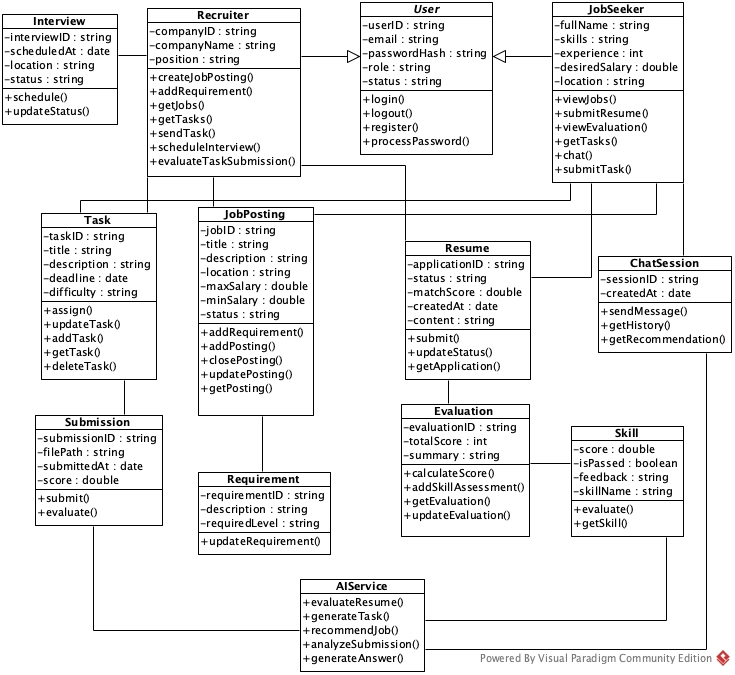
\includegraphics[scale=0.6]{Figures/chapter2/Analysis class diagram.jpg}
    \caption{Шинжилгээний класс диаграмм}
    \label{fig:sh-class}
\end{figure}

\section{Шинжилгээний дарааллын диаграмм}
\paragraph{}
Шинжилгээний класс диаграммд тодорхойлсон классуудын операторуудыг ашиглан \say{бүртгүүлэх}, \say{анкет илгээх болон AI үнэлгээ хийх}, \say{чатботтой харилцах} гэсэн үндсэн юзкейсүүдэд шинжилгээний шатны дарааллын диаграммыг гаргасан.

\par \noindent
Зураг \ref{fig:burtgel-zh-1} -д хэрэглэгч системд бүртгэл үүсгэх дарааллыг харуулж байна. Зочин бүртгэлийн форм бөглөж илгээхэд систем мэдээллийг шалгаж, давхардал байхгүй бол шинэ хэрэглэгчийн данс үүсгэнэ.
\begin{figure}[H]
    \centering
    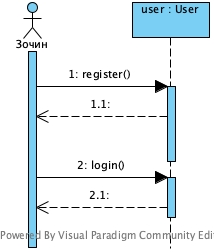
\includegraphics[scale=0.6]{Figures/chapter2/register.jpg}
    \caption{Бүртгэл үүсгэх шинжилгээний дарааллын диаграмм}
    \label{fig:burtgel-zh-1}
\end{figure}

\par \noindent
Зураг \ref{fig:submitResume} -д анкет илгээх болон AI үнэлгээ хийх дарааллыг харуулж байна. Ажил горилогч CV файлаа илгээхэд систем файлыг хадгалж, ажлын байрны мэдээлэлтэй хамт Claude API-д дамжуулна. Claude API тохирсон/дутуу ур чадвар болон нийт оноо агуулсан JSON хариулт буцаахад систем үр дүнг өгөгдлийн санд хадгалж, хэрэглэгчид харуулна.
\begin{figure}[H]
    \centering
    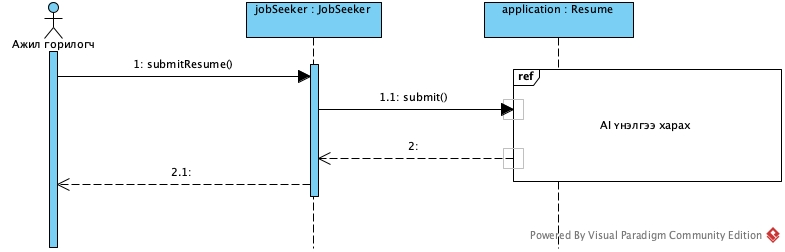
\includegraphics[scale=0.5]{Figures/chapter2/submitResume.jpg}
    \caption{Анкет илгээх шинжилгээний дарааллын диаграмм}
    \label{fig:submitResume}
\end{figure}

\begin{figure}[H]
    \centering
    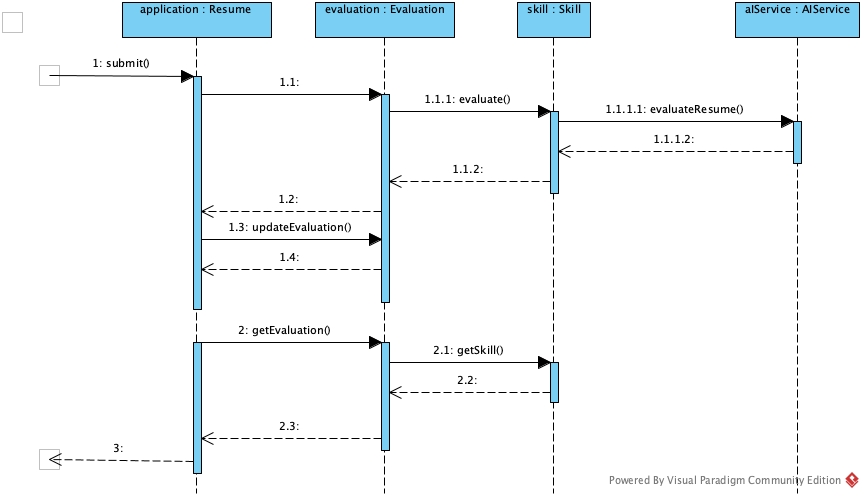
\includegraphics[scale=0.5]{Figures/chapter2/evaluation.jpg}
    \caption{AI үнэлгээ хийх шинжилгээний дарааллын диаграмм}
    \label{fig:eval}
\end{figure}
\par \noindent


\section{Үйл ажиллагааны диаграмм}
\paragraph{}
Системийн юзкейс диаграммд тодорхойлогдсон юзкейсүүдийн эхлэлээс төгсгөл хүртэлх үйлдлүүдийг дүрсэлсэн үйл ажиллагааны диаграммуудыг доор харуулав.
\par \noindent
Ажил горилогч анкет илгээх үйл ажиллагаа нь дараах дарааллаар явагдана: хэрэглэгч системд нэвтэрсний дараа сонирхсон ажлын байрны дэлгэрэнгүй хуудсыг нээнэ. "Анкет илгээх" товчийг дарж PDF файлаа сонгон илгээнэ. Систем файлыг хүлээн авч серверт хадгалаад, ажлын байрны шаардлагатай хамт AI-д дамжуулна. AI үнэлгээ дуусмагц хэрэглэгч оноо, тайлбар болон зөвлөмжийг харах боломжтой болно. Дээрх процессыг Зураг \ref{fig:sh_activity} -д харуулав.
\begin{figure}[H]
    \centering
    \includegraphics[scale=0.65]{Figures/chapter2/sh_activity.jpg}
    \caption{Анкет илгээх үйл ажиллагааны диаграмм}
    \label{fig:sh_activity}
\end{figure}
\par \noindent

\section{Бүлгийн дүгнэлт}
\paragraph{} Энэ бүлэгт системийн үйл ажиллагааг дэлгэрэнгүй тайлбарлаж, системийг ашиглах хэрэглэгчид болон шаардлагуудыг тодорхойлж, юзкейс, юзкейсийн тодорхойлолт болон шинжилгээний шатны класс, дараалал, үйл ажиллагааны диаграммуудыг гаргасан. Эхлээд системийг хэрэглэх хэрэглэгчдийг (ажил горилогч, ажил олгогч, зочин) тодорхойлоод оролцогч тал бүрийн функциональ шаардлагыг тодорхойлж, мөн системийн функциональ бус шаардлагыг ч тодорхойлсон. Системд оролцогчдын функциональ шаардлага дээр үндэслэн 3 тоглогч, 12 юзкейс бүхий юзкейс диаграммыг байгуулж, юзкейс бүрд тодорхойлолт гаргасан. Шинжилгээний шатны үндсэн классуудыг (Хэрэглэгч, Ажлын байр, Анкет, Даалгавар, Даалгаврын илгээлт, AI клиент) гаргаж, тэдгээрийн холбоо хамаарлыг тодорхойлсон. Тодорхойлогдсон классууд болон юзкейсийн тодорхойлолтын дагуу дарааллын диаграмм болон үйл ажиллагааны диаграммуудыг гаргаж, системийн үйл ажиллагаа, оролцогч талууд, процессын дарааллыг шинжилгээний түвшинд ойлгох боломжийг олгосон.